\chapter{Experimentos de campo}

\label{Capitulo_4}
\label{ExperimentoReal}
\section{Perfilado preliminar con \textbf{“\textit{steps}”}}
\subsection{Implementación}
\begin{figure}[!htb]
	\centering
	\includegraphics[width=0.7\textwidth]{Figuras/infraestructure/arduino-rpi.png}
	\captionsetup{margin=2cm}
	\caption[Flujo de datos en mediciones de perfilado]{Flujo de datos en mediciones de perfilado. El Arduino transfiere los datos mientras llegan directamente a la \acs{rpi} mediante \acs{usb}. Estos se agrupan por distancia (ingresada por el usuario) gracias al script de captura.}
	\label{fig:infra-diagram-arduino}
\end{figure}
\begin{figure}[!htb]
	\centering
	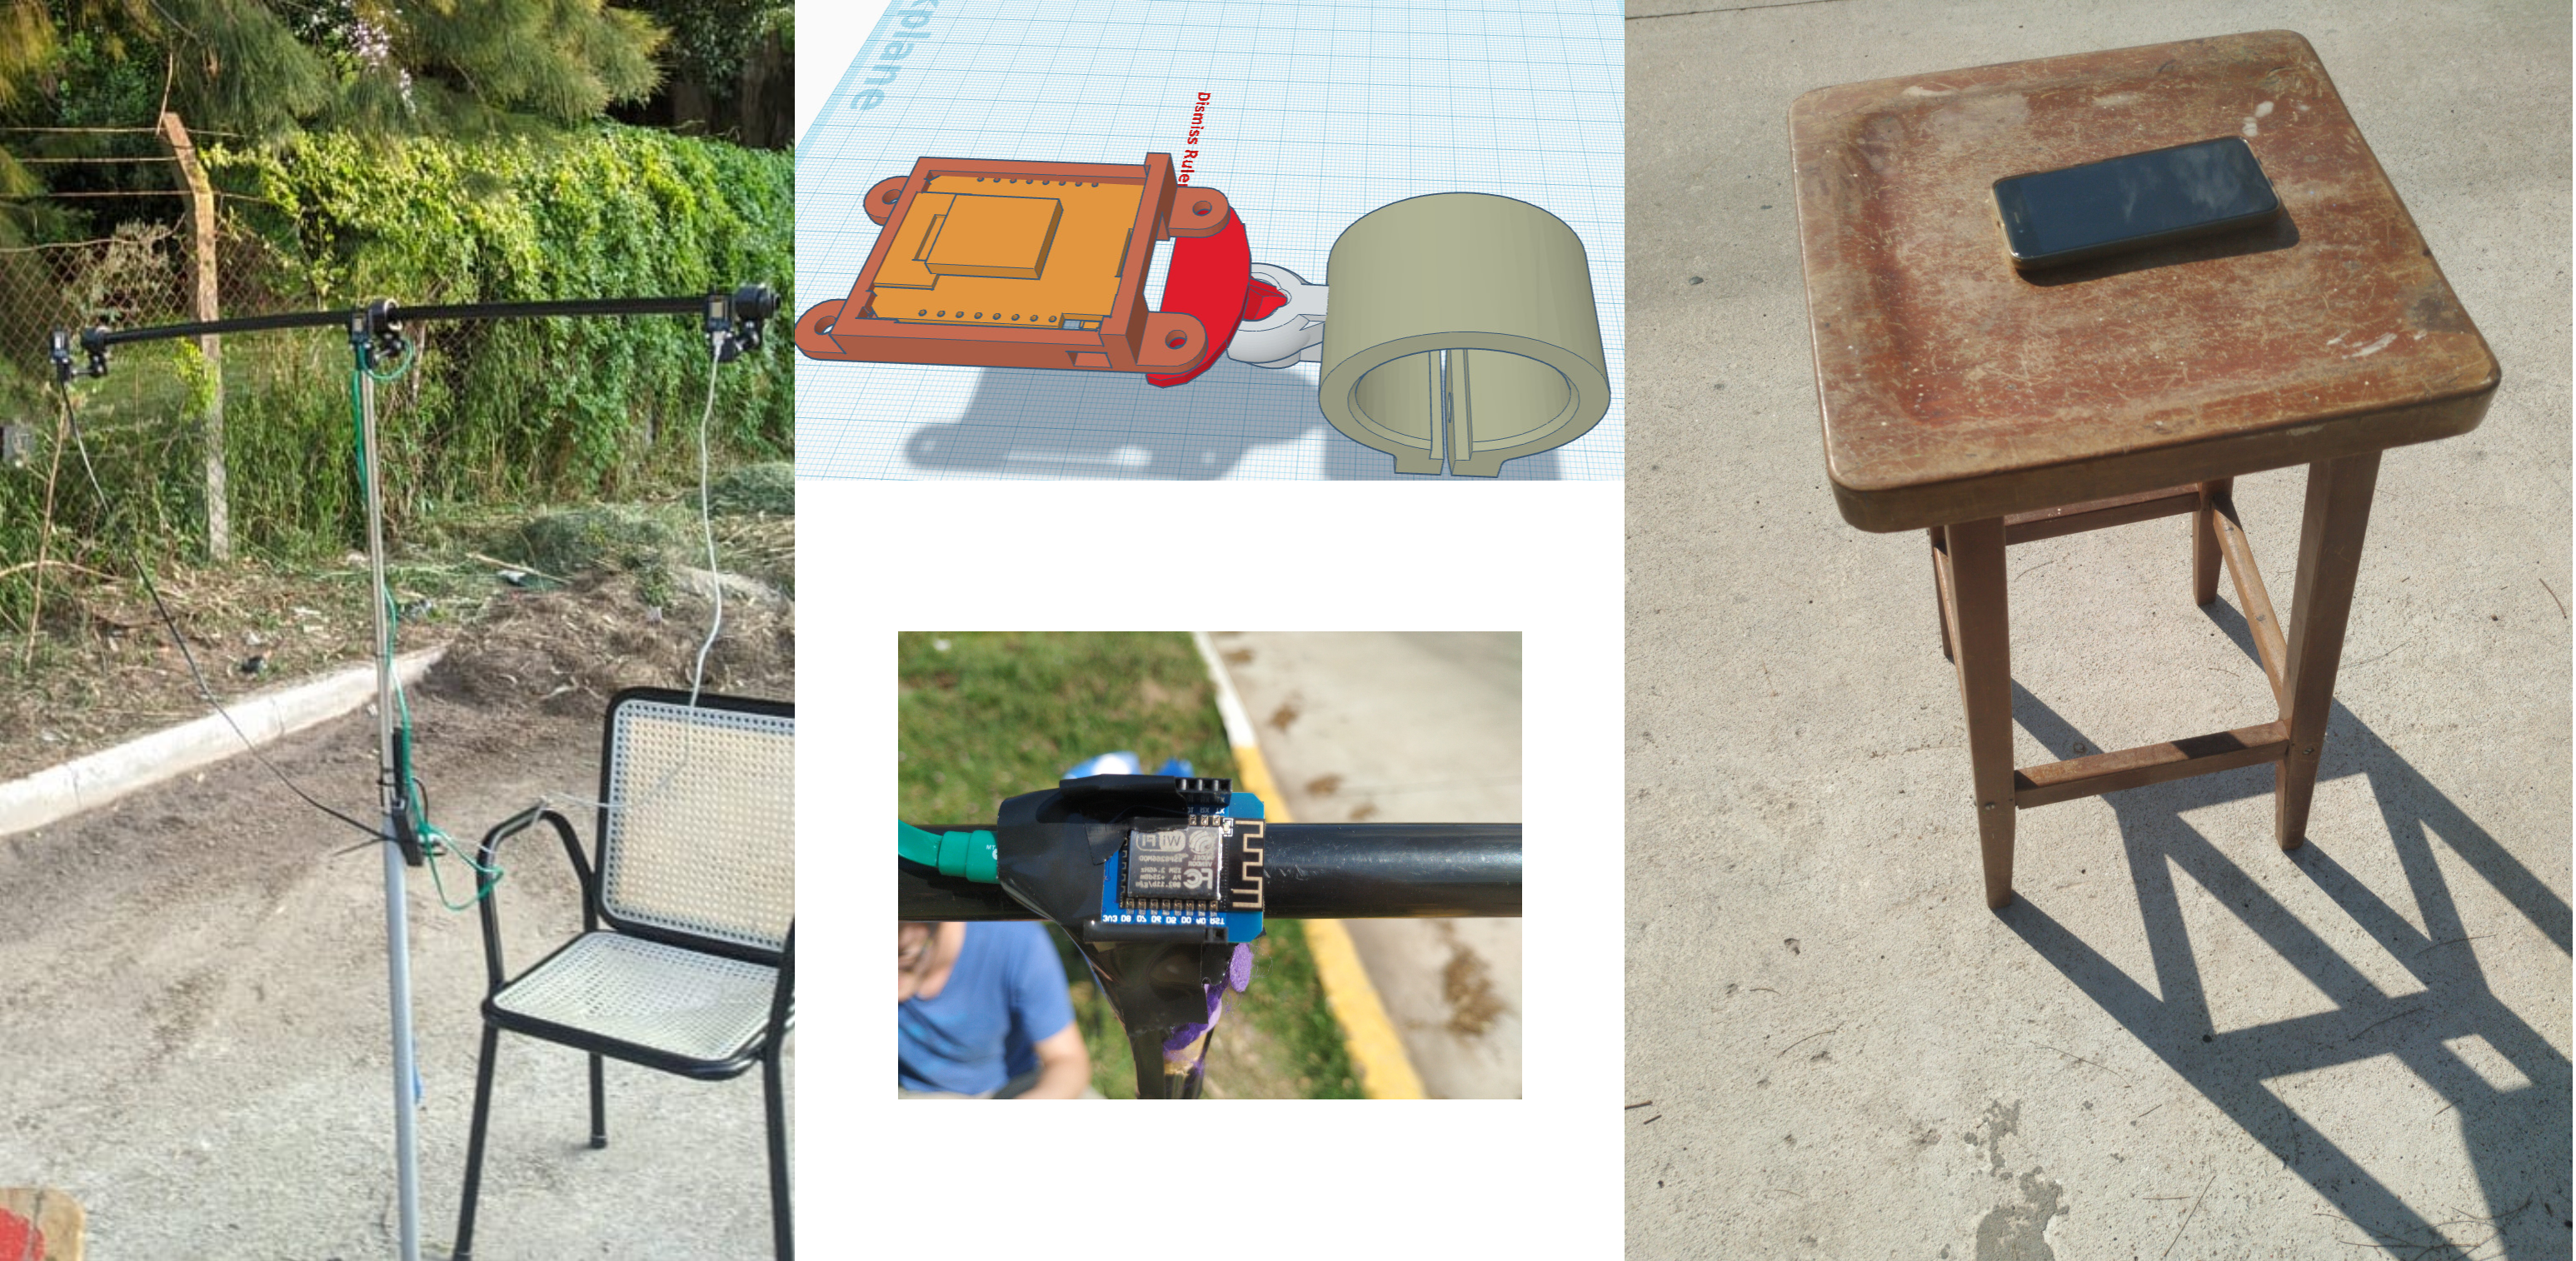
\includegraphics[width=0.8\textwidth]{Figuras/fieldwork/profiling-setup.png}
	\captionsetup{margin=2cm}
	\caption[Perfilado]{Experimento de campo de perfilado. Para que todos los dispositivos tengan sus antenas orientadas en el
mismo ángulo hacia la misma ubicación durante todo el experimento se utilizó
un soporte de metal con monturas hechas con impresora 3D.}
	\label{fig:arduino-profiling-setup}
\end{figure}

Antes de avanzar con los experimentos de campo hacia la etapa de multilateración, se quiso confirmar primero que la relación \acs{rssi} a distancia que informaban los \acs{esp} se acercaba a la realidad (es decir que se aproxime a lo que debería ser el ideal, o el modelo de \textit{Path Loss} antes visto). Similar a lo realizado en el experimento simulado pero con más nodos \textbf{Sniffer} para garantizar precisión.

Si bien se eligió utilizar una infraestructura \textit{wireless} más adelante como se describe en la sección \ref{sssec:num1}, primero se realizó un experimento preliminar cableado conectando tres \acs{esp} mediante \acs{usb} a una computadora \acl{rpi} para tomar múltiples muestras a una distancia conocida y poder poner un corte entre muestra y muestra a medida se recibíamos. De esta manera poder etiquetar múltiples muestras a 2 metros, a 5, a 10, etc.

Para recibir esta información se desarrolló un \href{https://github.com/agusalex/PacketSnifferServer}{script} que toma \textbf{M} muestras y luego se detiene a esperar a que el usuario le indique la nueva distancia en la que se realizará la próxima medición. De esta manera se obtiene \textbf{M} muestras agrupadas por la distancia, a esto le llamamos “\textit{step}”.


Además se decidió hacer el experimento de perfilado en un ambiente controlado (en el campo de deportes de la \acs{ungs} con muy poca interferencia en la banda 2.4 GHz). Se garantizó la precisión de los datos mediante la toma de 200 muestras por cada “\textit{step}” de medición. Y se realizaron 21 mediciones por cada dispositivo a 4.5 metros de distancia entre cada una. Dos de los dispositivos finalizaron el experimento, pero uno sufrió un desperfecto y dejó de recibir.
 
\begin{figure}[!htb]
	\centering
	\includegraphics{Figuras/fieldwork/profiling.png}
	\captionsetup{margin=2cm}
	\caption[Perfilado]{Experimento de perfilado en el campo de deportes de la UNGS}
	\label{fig:arduino-profiling-setup}
\end{figure}
 Como transmisor se utilizó un dispositivo móvil en modo \acs{ap} para poder obtener una visión precisa del comportamiento de la señal.

Para procesar los datos de \acs{rssi}, primero se realizó un filtrado \textit{Kalman} de la captura entera por dispositivo, como se puede observar en la figura \ref{fig:filtrado-kalman}. Como último paso, calculamos la media por cada “\textit{step}” de distancia para filtrar las anomalías de los datos. Finalmente se ejecutó una regresión logarítmica usando cuadrados mínimos, el resultado nos da un \textbf{A} y un \textbf{N} que podría ser utilizado en el paso de multilateración.

\subsection{Experimento}
%\begin{figure}[!htb]
%	\centering
%	\includegraphics[width=0.8\textwidth]{Figuras/profiling/device1/device1_regression.png}
%	\captionsetup{margin=2cm}
%	\caption[Media de \acs{rssi} segregado por distancia de la medición vs regresión logarítmica, prueba de campo]{Media de \acs{rssi} segregado por distancia de la medición vs regresión logarítmica, prueba de campo con \textit{steps}”, con ESP8266 en campo de deportes UNGS. Se hallaron valores para \textbf{A=37}, \textbf{N=21} y \textbf{R(residual)=89\ }}
%	\label{fig:dev1-regression}
%\end{figure}

La figura \ref{fig:dev2-dev1-regression} muestra los resultados obtenidos de este experimento de campo. En el eje X se puede observar la distancia real desde el dispositivo \acs{esp} hasta el dispositivo móvil transmisor en metros, mientras que en el eje Y se representa el RSSI medido. Cada punto en el gráfico representa una medición individual del \acs{rssi} en una determinada distancia.



\subsection{Conclusión}

Puede observarse que a medida que la distancia aumenta, el \acs{rssi} se ajusta a una curva según lo predicho por el modelo, lo que se alinea con lo que esperaríamos de la pérdida de señal en función de la distancia en un entorno con mínima interferencia. Sin embargo, también se pueden identificar algunas variaciones y anomalías en los datos, posiblemente debido a factores ambientales no controlados o a variaciones inherentes en la recepción de la señal.
\begin{figure}
	\centering
	\includegraphics[width=1\textwidth]{Figuras/profiling/preliminar-experiment.jpg}
	\captionsetup{margin=2cm}
	\caption[Media de \acs{rssi} segregado por distancia de la medición vs regresión logarítmica, prueba de campo]{Media de \acs{rssi} segregado por distancia de la medición vs regresión logarítmica, prueba de campo con “\textit{steps}”, con ESP8266 en campo de deportes UNGS. Se hallaron valores del dispositivo 1 para \textbf{A=37}, \textbf{N=21} y \textbf{R(residual)=89}
    Para el dispositivo 2 \textbf{A=49}, \textbf{N=18} y \textbf{R(residual)=88}}
\label{fig:dev2-dev1-regression}
\end{figure}
Finalmente, realizamos una regresión logarítmica para obtener una representación ajustada de la relación entre la distancia y el \acs{rssi}. El resultado de esta regresión nos proporcionó los parámetros \textbf{A} y \textbf{N} para cada dispositivo, al igual que en el experimento simulado.




\section{Infraestructura de pruebas de campo \textit{wireless}} \label{sssec:num1}

\begin{figure}[!htb]
	\centering
	\includegraphics[width=0.8\textwidth]{Figuras/infraestructure/arduino-rpi-multi.png}
	\captionsetup{margin=2cm}
	\caption[Flujo de datos en mediciones de multilateración]{Flujo de datos en mediciones de multilateración. Los Arduinos recolectan los datos hasta agotar el espacio en memoria o llegar a un límite establecido. Finalmente descargan toda la información en una \acs{rpi} de manera inalámbrica.}
	\label{fig:infra-diagram-arduino}
\end{figure}

Se plantearon distintas alternativas de \textit{hardware} para poder cubrir el área más grande posible al menor costo. Se pensó en la utilización de \textit{routers} comerciales como los \textit{Ubiquiti} usando un software de código abierto como \textit{OpenWRT}, también la posibilidad de usar \acl{rpi} o similares e incluso microcontroladores con \acs{wifi} compatibles con Arduino como el \acs{esp} y el \acs{esp32}.

Cualquiera de estas soluciones trae consigo un problema ineludible: Los adaptadores \acs{wifi} hasta donde hemos podido investigar no pueden operar en modo promiscuo en simultáneo mientras que opera en otro modo, por ejemplo, en modo \acl{ap} o modo cliente mientras se encuentra en modo promiscuo. Se planteó la posibilidad de usar dispositivos que cuentan con dos adaptadores de \acs{wifi}, uno para capturar paquetes \acl{prq} y otro para evacuarlos hacia una base de datos centralizada para que luego puedan ser analizados pero no se encontró ninguno de bajo costo y de uso masivo.

Por esto fue elegida la alternativa de utilizar muchos dispositivos \acs{esp} como \textit{Sniffer} y un \textit{\acl{rpi} 3} en modo \textit{Access Point} para recibir los datos. Para facilitar las mediciones a modo de soporte aseguramos cada \textit{Sniffer} a un tubo de PVC con una base de cemento. Los \acs{esp} fueron adheridos con \textit{velcro} al tubo y se le agregó una batería de LI-ION conectada a los pines \acs{vin} y \acs{gnd} del dispositivo como se puede observar en la imagen \ref{fig:infra-diagram-arduino}.

El \acs{esp} fue programado utilizando Arduino y Platformio para el sensor y Python para el server que recibe los datos. Se configuró el dispositivo en modo promiscuo y se procedió a capturar paquetes y descomponer los \textit{Beacon Frames} en sus parámetros utilizando el \textit{SDK} del \acs{esp}. De dicho \textit{frame}, parte del 802.11, se extrae puntualmente el \acs{rssi}, \acs{mac} y el número de secuencia del paquete.

Se configuró el \acs{esp} para conectarse a una red Wi-Fi emitida por una \textit{\acl{rpi}} (configurada en modo \textit{AP} para facilitarnos la infraestructura de red) y enviar a la \acl{rpi} vía \acs{udp} los paquetes agregados de a grupos de \textbf{N} paquetes donde \textbf{N} es el máximo número que se podía enviar sin llenar el \textit{frame} de \acs{udp}. De esta manera optimizamos el tiempo de envío ya que múltiples nodos enviando a la vez de a un paquete pequeño por vez vía \acs{wifi} tendían a sobrecargar a la red y a la \acs{rpi} que necesita procesar y escribir los datos en una tarjeta SD.
La \textit{\acl{rpi}} contenía un script que recibe los datos \acs{udp} de cada nodo, y guarda en un solo archivo CSV la siguiente información: \textbf{ip\_sniffer}, \textbf{rssi}, \textbf{num\_secuencia}. Luego ese archivo se descarga manualmente conectándose por SSH a la \acs{rpi}.

El número de secuencia se emplea como un identificador único para cada paquete, permitiendo su agrupación durante la realización de experimentos de multilateración o perfilado, similar a cómo se agruparon los paquetes por milisegundos de captura en los experimentos simulados. Este método elimina la necesidad de mantener relojes sincronizados entre los nodos, como sería necesario si se usaran los milisegundos de captura como criterio de agrupación. Sincronizar relojes en un entorno de infraestructura \textit{wireless} representaría un desafío considerable que se decidió evitar.
De esta manera, al analizar un paquete, podemos identificarlo con certeza y comparar de manera inequívoca los \acs{rssi} recibidos y la diferencia entre estos para cada \textit{Sniffer}.

Finalmente, una vez capturadas suficientes tuplas de (\textbf{número\_secuencia}, \textbf{rssi}) descartando las que no sean de la \acs{mac} de nuestro \textit{Objetivo}, los dispositivos cortan la recepción antes de llenar la limitada memoria del dispositivo, este proceso suele durar 2 minutos aunque varía según la tasa de transmisión de paquetes del \textit{Objetivo}. Luego los \acs{esp} proceden a agregar las tuplas capturadas y enviarlas de a grupos mediante \acs{udp} hacia la \acs{rpi}. Esta última recopila los datos y les agrega la \acs{ip} de cada \textit{Sniffer} para poder identificar de dónde vino la información para luego ser procesada. Finalmente se persiste en un archivo CSV.

Como nodo \textit{Objetivo} se utilizó un teléfono celular en modo \acl{ap} para incrementar la tasa de transmisión de paquetes. De esta manera nos limitamos a capturar los paquetes de tipo \textit{Beacon Frame} que emite el teléfono usando su \acs{mac} como filtro. Consideramos que es un buen equivalente a una situación donde un transeúnte cuenta con un teléfono sin estar en modo \acl{ap} pero emitiendo \acl{prq}. Esto, con la salvedad de la Mac Address Randomization y la escasa frecuencia de emisión de los \acl{prq}, lo que no lo haría beneficioso para este experimento.

\section{Interferencias y Rango Usable para Multilateración con ESP8266}
\begin{figure}[!htb]
	\centering
	\includegraphics[width=0.95\textwidth]{Figuras/errores/estatico-medio.jpg}
	\captionsetup{margin=1cm}
	\caption[ Experimento estático]{ Experimento estático, misma disposición de nodos que el de multilateración. Se pueden observar grandes variaciones por interferencia del ambiente en el experimento sin movimiento. Los filtros de Kalman ayudan a mejorar esto.}
	\label{fig:errores-estatico}
\end{figure}
\subsection{Experimento estático}

 Utilizando la técnica de captura \textit{stepless} ya descrita se colocó un teléfono móvil a 15 metros de los nodos, los cuales se dispusieron en línea recta uno al lado del otro al igual que en el experimento de perfilado.
 Luego, sin mover el móvil, se procedió a capturar paquetes hasta completar la medición.
 Como se puede observar en la figura \ref{fig:errores-estatico} algunos nodos capturaron más datos que otros. Esto se debe a que durante la medición algunos nodos experimentaron fallos intermitentes en la alimentación, lo que provocó interrupciones en la recepción de señal. Durante la medición, algunos nodos experimentaron fallos intermitentes en la alimentación debido a un suministro de voltaje inadecuado. Esto ocurrió porque los nodos fueron alimentados directamente desde una batería de iones de litio con un voltaje nominal de 3.7V y un máximo de 4.2V, lo cual es insuficiente para el regulador AMS1117-3.3 integrado en la placa. Este regulador requiere un mínimo de 4.5V para operar correctamente; al no recibir un voltaje adecuado, la tensión de salida fluctuó por debajo de los 3.3V requeridos por el ESP8266, provocando estados inestables en su ejecución. Como resultado, algunos nodos dejaron de recibir paquetes al quedar en un estado de bloqueo (\textit{hang state}) o reiniciarse inesperadamente. Este problema afectó la consistencia de la captura de datos, generando discrepancias en la cantidad de paquetes registrados por cada nodo.

Otros experimentaron grandes interferencias, variando así por varios metros una potencial predicción de distancia.

 En todas las gráficas se puede ver cómo el filtro de Kalman ayuda a reducir el ruido y se adapta a los cambios en el perfil de recepción de la señal que persisten en el tiempo.
 Dicho filtro resultará una herramienta fundamental para mejorar la precisión en los experimentos subsiguientes.

\subsection{Precisión en el perfilado}


Luego de realizar varios experimentos de perfilado quedó en evidencia el problema que surge del modelo de \textit{Path Loss}: A medida que la distancia aumenta, la precisión baja considerablemente. Esto se puede observar en la figura \ref{fig:distance-error-range}, donde en la gráfica de la izquierda podemos observar cómo dada una posible interferencia temporal en la medición, la media de \acs{rssi} recibida a 12.5 metros es igual a la predicha por el ajuste logarítmico a 19 metros, en total un error de 6.5 metros. Lo que es más aún, la media de \acs{rssi} a 12.5 metros es igual a la media recibida a aproximadamente 25 metros, en total un error de 12.5 metros. Claramente, incluso a cortas distancias de menos de 20 metros se pueden ver distorsiones enormes en la distancia predicha. Continuando con este análisis, si consideramos la gráfica derecha en la misma figura, la cota inferior del desvío estándar (stdev-) a 27 metros es igual a la cota superior del desvío a 51 metros, en total, 24 metros de error entre ambos desvíos.

\begin{figure}[!htb]
	\centering
	\includegraphics[width=0.95\textwidth]{Figuras/errores/4-raw-compilation-annotated.png}
	\captionsetup{margin=1cm}
	\caption[Variación de la distancia con \acs{rssi}]{Variaciones en la media y los desvíos estándar demuestran la poca precisión de estos dispositivos en distancias de más de 10 metros.}
	\label{fig:distance-error-range}
\end{figure}
\begin{figure}[!htb]
	\centering
	\includegraphics[width=0.95\textwidth]{Figuras/errores/distance_percentage_increase.png}
	\captionsetup{margin=1cm}
	\caption[Variación de la distancia con \acs{rssi}]{Variación de la distancia estimada por cada incremento de 1 dBm en \acs{rssi}, demostrando la precisión dentro de un rango de 10 metros y la creciente inexactitud más allá de este límite.}
	\label{fig:distance-percentage-increase}
\end{figure}

Por estos motivos se determinó que el rango usable efectivo de los dispositivos \acs{esp}, para experimentos de multilateración enfocados en identificar patrones de movimiento, es de hasta 10 metros. Incluso si se toma el modelo de \textit{Path Loss} sin interferencia como referencia, como podemos ver en la figura \ref{fig:distance-percentage-increase}, podemos observar que a partir de los 10 metros, por cada 1 dBm de variación en la intensidad de la señal \acs{rssi} se traducirá en cambios de aproximadamente 1 metro en la distancia estimada.

Este rango se ha demostrado adecuado para experimentos donde se buscaba determinar patrones de movimiento específicos, como patrones en forma de estrella o cuadrados, dentro de áreas confinadas. La elección de limitar las pruebas a una cuadrícula de 10x10 metros surgió tras experimentos multilaterales fallidos en áreas más extensas, como cuadrículas de 25x25 metros, donde el aumento de la imprecisión en las estimaciones de distancia comprometía la fiabilidad de los resultados.

Sin embargo, es importante destacar que el rango usable de 10 metros identificado en nuestra investigación es específico, primero, para el perfil de recepción de estos dispositivos y, segundo, puntualmente para la detección de patrones de movimiento detallados mediante multilateración. Para otros objetivos, como detección de presencia en áreas más amplias, el rango usable podría extenderse aún más. Y si consideramos el uso de antenas de mayor ganancia o la implementación de una mayor cantidad de dispositivos para cubrir un área mayor, este rango podría ser aún mejor.


\section{Perfilado sin \textbf{\textit{steps}}}

A pesar de los resultados prometedores obtenidos en los experimentos preliminares de perfilado, se hizo evidente que el perfilado es específico para cada sensor en un ambiente determinado. Esto se debe a que la curva de atenuación de la señal, que describe cómo disminuye la intensidad de la señal a medida que el transmisor se aleja, depende en gran medida del ruido ambiental del lugar donde se realice el experimento y de las características propias de cada dispositivo.

\begin{figure}[!htb]
    \centering
    \includegraphics[width=0.8\textwidth]{Figuras/fieldwork/combined.png}
    \captionsetup{margin=2cm}
    \caption[Postes de Nodo Multilateración]{A la izquierda: Nodos \textit{Sniffer} construidos con PVC y una base de cemento. El ESP8266 fue adherido con velcro al tubo junto con una batería de LI-ION. A la derecha, un acercamiento a uno de los nodos notando donde se conectó el ESP8266 a la batería utilizando los terminales 5V y GND.}
    \label{fig:infra-diagram-arduino}
\end{figure}
Con el objetivo de evaluar la capacidad para predecir movimientos de un individuo en un ambiente urbano, y ante las limitaciones de acceso al campo de deportes de la \acs{ungs}, se optó por realizar experimentos en el campus de la \acs{ungs}, un lugar de alta concurrencia y con potencial interferencia de señal debido a la presencia de edificios. Del cual podíamos disponer en cualquier momento y así realizar más experimentos.

\begin{figure}[!htb]
    \centering
    \includegraphics[width=0.95\textwidth]{Figuras/profiling/stepless.png}
    \captionsetup{margin=1cm}
    \caption[Stepless]{Resultados de perfilado \textit{stepless}.}
    \label{fig:stepless}
\end{figure}
Se decidió además probar el método de captura \textit{wireless} descrito en la sección \ref{sssec:num1} en un escenario de perfilado conocido antes de avanzar a la etapa de multilateración, con el fin de integrar todos los componentes de este trabajo. Este método no solo facilita la realización del experimento de perfilado, sino que también se asemeja más al escenario final de multilateración que se empleará posteriormente.

El término \textit{stepless} hace referencia a un enfoque de perfilado que no requiere de los pasos discretos predefinidos en términos de distancia conocida durante la captura de datos. En lugar de establecer intervalos fijos de distancia para la toma de mediciones, este método permite una captura continua a medida que el \textbf{Objetivo} se mueve a través del espacio. No obstante, para poder utilizar las ya mencionadas herramientas de perfilado, todavía se generan "pasos" virtuales basados en el tiempo y la secuencia de los paquetes capturados, lo que permite estimar la distancia recorrida. Estos pasos generados no corresponden a agrupaciones discretas con distancias conocidas, sino que son el resultado de una estimación que utiliza la secuencia de paquetes, la velocidad de movimiento y la frecuencia de transmisión del dispositivo móvil, facilitando así un análisis detallado sin la necesidad de mediciones de distancia fijas y conocidas previamente.

\subsection{Experimento}


A diferencia del experimento preliminar de perfilado realizado en el campo de deportes, este experimento se llevó a cabo en el campus de la UNGS.

Se dispusieron múltiples nodos en línea perpendicular al recorrido, formando una T con este, y se procedió a alejarse hasta alcanzar los 75 metros. Una vez completado el recorrido, se esperó a que los nodos finalizaran la captura y descarga de datos.

El método de captura \textit{wireless} empleado consiste en caminar a velocidad constante desde el punto donde se ubican los sensores, tomando nota del tiempo transcurrido hasta alcanzar una distancia determinada (por ejemplo, 30 metros en 30 segundos), mientras los sensores capturan los paquetes. Una vez finalizado el experimento, los datos se almacenan en la \acs{rpi}.

Dado que el dispositivo móvil utilizado (Samsung S20) emite paquetes cada 150 ms y conocemos el número de secuencia de cada paquete, es posible estimar la distancia a la que fue capturado y agruparlos en \textit{steps} discretos de distancia. Aunque se pierde precisión en la distancia exacta de captura, este agrupamiento y el cálculo del promedio mitigan el potencial error.

\subsection{Conclusiones}

El perfilado sin \textit{steps} permitió realizar experimentos de manera más rápida, facilitando la obtención de los valores de \(N\) y \(A\) en diferentes ambientes y para múltiples nodos simultáneamente, sin necesidad de conexión por cable o de tomar notas manuales sobre las distancias, reduciendo el tiempo de medición de 1 hora a 15 minutos. Además, se posiciona como una opción ideal para el despliegue rápido de nodos en un nuevo ambiente. Como se muestra en la figura \ref{fig:stepless}, se logró determinar los valores de \(N\) y \(A\) para cada sensor.

No obstante, algunos sensores presentaron interferencias significativas o su recepción se detuvo abruptamente, un problema recurrente a lo largo de este trabajo. La variabilidad observada en un experimento estático sin movimiento sugiere posibles defectos en los nodos o interferencias en el área de experimentación que afectaron a algunos nodos más que a otros, como se ilustra en la figura \ref{fig:errores-estatico-medio}.


\section{Multilateración}

\begin{figure}[!htb]
    \centering
    \includegraphics[width=0.6\textwidth]{Figuras/infraestructure/infra-diagram.png}
    \captionsetup{margin=2cm}
    \caption[Flujo de datos]{Flujo de datos en el experimento de multilateración.}
    \label{fig:infra-diagram}
\end{figure}
\begin{figure}[!htb]
	\centering
\includegraphics{Figuras/fieldwork/trilateration.png}
	\captionsetup{margin=2cm}
	\caption[Perfilado]{Experimento de perfilado en el campus de la UNGS}
	\label{fig:arduino-profiling-setup}
\end{figure}
\subsection{Infraestructura}

De manera similar al experimento de perfilado, se implementó una red de nodos \textbf{Sniffer} en el campus de la \acs{ungs}, siguiendo un esquema predeterminado. En este caso, se colocaron ocho nodos formando un cuadrado de 10 x 10 metros. Estos nodos se dedicaron a monitorear las señales Wi-Fi, capturando la intensidad de la señal \acs{rssi} emitida por el nodo \textbf{Objetivo}, que se desplazaba siguiendo una ruta preestablecida dentro del alcance de los nodos \textbf{Sniffer}. Durante el experimento, el nodo \textbf{Objetivo} mantuvo una velocidad constante.

Los nodos \textbf{Sniffer} registraron la \acs{rssi} de las señales emitidas por el nodo \textbf{Objetivo}, junto con el número de secuencia de cada señal, transmitiendo estos datos a una \acl{rpi} mediante Wi-Fi, una vez completado el experimento y llenados sus buffers para el posterior análisis de los datos.

Con los valores de \textbf{A} y \textbf{N} derivados de los experimentos de perfilado previos y utilizando la fórmula que convierte el valor de \acs{rssi} en distancia, se estimó la separación entre cada nodo \textbf{Sniffer} y el nodo \textbf{Objetivo} para cada paquete con el mismo número de secuencia. Se realizaron un mínimo de cinco mediciones de distancia con distintos nodos para cada punto en el tiempo para garantizar una mayor precisión.

Si bien durante la etapa de perfilado, se calculó un \textbf{A} y un \textbf{N} distintos para cada nodo. Tal como se discutirá más adelante, las interferencias fueron un factor muy importante durante las pruebas en el campus de la \acs{ungs}. Muchos nodos arrojaron valores muy distintos simplemente por los grandes cambios en la señal, incluso estando quietos, como se aprecia más adelante en la figura \ref{fig:errores-estatico}. Por este motivo, se eligieron los valores de \textbf{A} y de \textbf{N} del experimento de perfilado que mejor ajuste tuvo, es decir que tuvo menor residual.
En este caso \textbf{A=43} y \textbf{N=31}.

\begin{figure}[!htb]
\centering
\includegraphics[width=0.8\textwidth]{Figuras/multilateration/multilateration_star.png}
\captionsetup{margin=2cm}
\caption[Configuración de la multilateración en Tiempo Real]{Configuración del experimento de multilateración en tiempo real en el campo de deportes de la \acs{ungs}.}
\label{fig:real-multilateration}
\end{figure}

\begin{figure}[!htb]
\centering
\includegraphics[width=0.8\textwidth]{Figuras/multilateration/multilateration_square.png}
\captionsetup{margin=2cm}
\caption[Resultados de la multilateración en Tiempo Real]{Resultados de la multilateración en tiempo real, mostrando la trayectoria estimada del nodo \textbf{Objetivo} en comparación con su trayectoria real.}
\label{fig:real-multilateration-results}
\end{figure}


\subsection{Experimento}

Se llevaron a cabo múltiples recorridos en distintas ejecuciones de este experimento. Si bien durante el experimento se utilizaron 8 nodos, en la figura \ref{fig:real-multilateration} solo se representaron con círculos rojos 6 nodos. En la figura \ref{fig:real-multilateration-results} se puede ver que solo hay representados 5 nodos. Esto se debe a que algunos nodos presentaron altas interferencias y sus datos fueron descartados. También se debe a que algunos nodos no recibieron señal parcial o totalmente en algunos o todos los experimentos. Estos fenómenos serán explicados en más detalle en el capítulo \ref{Cap_Errores}.
La multilateración se llevó a cabo comparando las posiciones estimadas del nodo \textbf{Objetivo} con su trayectoria real, con el fin de evaluar la precisión de este método. Aunque los resultados mostraron cierto nivel de error en la estimación de la ubicación, estos se discutirán en detalle en la sección siguiente.


Las estimaciones de la ubicación obtenidas mediante la multilateración, representadas en las figuras \ref{fig:real-multilateration} y \ref{fig:real-multilateration-results}, se compararon con la trayectoria real del nodo \textbf{Objetivo} para evaluar la precisión del método. En los gráficos, los nodos \textbf{Sniffer} están ubicados en posiciones fijas, mientras que el nodo \textbf{Objetivo} sigue una ruta predeterminada.

Cada punto en los gráficos simboliza una estimación de la posición del nodo \textbf{Objetivo}, calculada a partir de las mediciones de \acs{rssi} recogidas por varios nodos \textbf{Sniffer}, el número de secuencia de los paquetes, y los parámetros \textbf{A} y \textbf{N} obtenidos de los experimentos de perfilado.

La línea azul ilustra la trayectoria real seguida por el nodo \textbf{Objetivo}, mientras que la línea verde muestra las estimaciones de su posición según la multilateración. Se puede observar que las estimaciones recrean levemente la trayectoria original, aunque presentan grandes deformaciones.


\subsection{Conclusión}

A pesar de las discrepancias y deformaciones observadas en las estimaciones de la ubicación del nodo \textbf{Objetivo}, el recorrido estimado mantiene cierta semejanza con la trayectoria original. Esto indica que, aunque existen errores significativos en la precisión de la localización, el enfoque de multilateración empleado logra capturar la esencia del movimiento del nodo \textbf{Objetivo} dentro del área de cobertura de los nodos \textbf{Sniffer}. Sin embargo, se identificaron zonas donde las estimaciones se alejaban significativamente de la trayectoria real, atribuibles a diversos factores como la interferencia inalámbrica, movimientos no intencionados del nodo \textbf{Objetivo}, y errores en la medición de \acs{rssi}.

Dentro de los resultados obtenidos, las discrepancias constantes en las estimaciones de ubicación, manifestadas como desplazamientos constantes o rotaciones en el gráfico, pueden deberse a múltiples factores relacionados con el entorno y la metodología de medición. Un desplazamiento constante en las estimaciones indica un sesgo sistemático en la medición del \acs{rssi}, posiblemente a causa de diferencias en la ganancia de las antenas de los nodos \textbf{Sniffer} o que la antena del nodo \textbf{Objetivo} no fuera precisamente omnidireccional (como no suelen serlo en teléfonos móviles).

Por otro lado, las rotaciones observadas en la predicción del recorrido, podrían deberse a personas en el camino de la señal o errores en la ubicación de los nodos, por ejemplo, un velcro flojo y un nodo que apunta ligeramente hacia un lado o al otro. Factores adicionales, como la reflexión de señales en superficies cercanas o la difracción a través de obstáculos también pueden contribuir a los errores y deformaciones registrados.